\documentclass[12pt]{article}
\usepackage{amsmath}
\usepackage{amsfonts}
\usepackage{float}
\usepackage{fancyhdr}
\usepackage{graphicx}
\usepackage{setspace}
\usepackage[colorlinks=true,linkcolor=blue,citecolor=red]{hyperref}
\usepackage{url}
\usepackage[top=.75in,left=.75in,right=.75in,bottom=1in]{geometry}
\usepackage{algorithm}
\usepackage{algpseudocode}
\usepackage{listings}
\usepackage{xcolor}
\usepackage{array}
\usepackage{longtable}
\usepackage{enumitem}
\usepackage{booktabs}
\usepackage{iftex}
\ifPDFTeX
\usepackage[T1]{fontenc}
\usepackage[utf8]{inputenc}
\usepackage{lmodern}
\else
\usepackage{fontspec}
\setmainfont{DejaVu Serif}
\setsansfont{DejaVu Sans}
\setmonofont{DejaVu Sans Mono}
\fi
\definecolor{codegreen}{rgb}{0,0.6,0}
\definecolor{codegray}{rgb}{0.5,0.5,0.5}
\definecolor{codepurple}{rgb}{0.58,0,0.82}
\definecolor{backcolour}{rgb}{0.95,0.95,0.92}
\lstdefinestyle{mystyle}{
  backgroundcolor=\color{backcolour},
  commentstyle=\color{codegreen},
  keywordstyle=\color{magenta},
  numberstyle=\tiny\color{codegray},
  stringstyle=\color{codepurple},
  basicstyle=\ttfamily\footnotesize,
  breakatwhitespace=false,
  breaklines=true,
  captionpos=b,
  keepspaces=true,
  numbers=left,
  numbersep=5pt,
  showspaces=false,
  showstringspaces=false,
  showtabs=false,
  tabsize=2
}
\lstset{style=mystyle}
\graphicspath{{./}}
\setlength{\emergencystretch}{3em}
\setlist[enumerate]{label=\arabic*.,leftmargin=*}
\setlist[itemize]{leftmargin=*}
\setlength{\headheight}{29.43912pt}
\pagestyle{fancy}
\fancyfoot{}
\fancyfoot[R]{Page \thepage}
\setlength{\parindent}{0pt}
\renewcommand{\baselinestretch}{1.5}
\newcommand{\coursename}{Introduction of Software Engineering}
\newcommand{\reportname}{Studitopia}
\newcommand{\reporttitle}{\href{https://github.com/RoundFloor/Studitopia.git}{Studitopia}}
\newcommand{\studentname}{%
Nguyen Thanh An (24125024)\\
Nguyen Chi Bao (24125025)\\
Tran Nguyen Khanh Binh (24125026)\\
Tran Canh Anh Tuan (24125048)\\
Nguyen Le Quoc Huy (24125100)
}
\newcommand{\teachername}{Ho Tuan Thanh, Nguyen Thi Minh Tuyen}
\lhead{\reporttitle}
\rhead{University of Science - VNUHCM\\
\coursename}
\newcommand{\leftfooter}{}
\lfoot{\leftfooter}
\begin{document}
\pagenumbering{arabic}

\section{17/11, Sprint 4 - Meeting Report}

\subsection{1. Team members present}

\begin{itemize}

\item Nguyen Thanh An

\item Nguyen Chi Bao

\item Tran Nguyen Khanh Binh

\item Nguyen Le Quoc Huy

\item Tran Canh Anh Tuan

\end{itemize}

No member is absent.

\subsection{2. Status reports}

\begin{longtable}{|p{0.24\linewidth}|p{0.24\linewidth}|p{0.24\linewidth}|p{0.24\linewidth}|}
\hline
Member & Completed Tasks & Issues & To-do Tasks \\
\endfirsthead
\hline
Member & Completed Tasks & Issues & To-do Tasks \\
\endhead
\hline
\endfoot
\hline
\endlastfoot
\textbf{Nguyen Thanh An} & - Render the Forum Home, area, subject and post page.\newline- Integrate the forum browsing and post search APIs into the frontend.\newline- Revise Verify university email features which loading infinitely in certain cases. & - Searched and filtered subject doesn't update when the data changes.\newline- Forum page router is inconsistent. & - Implement the post detail view, area page and subject page.\newline- Handle search/filter subjects consistently when the data changes.\newline- Fix the email verification features to avoid long-time loading. \\
\hline
\textbf{Nguyen Chi Bao} & - Write initial test cases for forum browsing, keyword search and tag filtering. & - Search relevance for AI-assisted recommendations is not deterministic yet.\newline- Tag-filter acceptance criteria need to be agreed before testing. & - Implement library, friend pages.\newline- Continue researching post recommendation input for the AI component. \\
\hline
\textbf{Tran Nguyen Khanh Binh} & - Design the Forum Home, post detail, tag filter, search result and interaction UI. & - Some card render the unnecessary information. & - Design the different cards for the unnecessary ones.\newline- Prepare the UI workflow and screen references for the PA4 document. \\
\hline
\textbf{Nguyen Le Quoc Huy} & - Implement APIs for forum browsing, area, subject and post retrieval. & - Search query parameters and pagination format are not yet consistent with the frontend.\newline & Implement APIs for post viewing, keyword search and tag filtering.\newline- Write the API contract section for recommend post, tag.\newline \\
\hline
\textbf{Tran Canh Anh Tuan} & - Revise the forum/post/comment/tag schema.\newline &  & - Add migrations for area, subject and post tables.\newline- Validate query plans for forum and post search.\newline- Update the relational schema section for post searching, relevant post retrieval. \\
\hline
\end{longtable}

\subsection{3. Summary of the meeting}

\subsubsection{3.1 Evaluate completed tasks}

\begin{itemize}

\item \textbf{Schema/Design foundation}: Tuan revised the forum/post/comment/tag schema; Binh completed UI designs for Forum Home, post detail, tag filter, search result, and interaction screens.

\item \textbf{API}: Huy implemented initial APIs for forum browsing, area, subject, and post retrieval.

\item \textbf{Frontend integration}: An rendered Forum Home, area, subject, and post pages, and integrated forum browsing and post search APIs; he also revised university email verification.

\item \textbf{Testing}: Bao wrote initial test cases for forum browsing, keyword search, and tag filtering.

\item \textbf{Outstanding issues}: forum router/search-filter refresh inconsistency, inconsistent search/pagination API contracts, unsettled tag-filter acceptance criteria, non-deterministic AI recommendation relevance, and some UI cards showing unnecessary information.

\end{itemize}

\subsubsection{3.2 To-do task}

\begin{itemize}

\item \textbf{Schema/Database}: add area/subject/post migrations, validate forum/post search query plans, and update relational schema for post search and relevant post retrieval (Tuan).

\item \textbf{API/Backend}: implement post viewing, keyword search, and tag filtering APIs; write recommend post/tag API contracts (Huy).

\item \textbf{Frontend integration}: implement post detail, area, and subject pages; fix search/filter data refresh and email verification loading; handle inconsistent forum routing (An). implement library, friends page (Bao)

\item \textbf{Testing/Validation}: validate API contracts with Huy before integration testing; continue AI recommendation research and expand test coverage (Bao).

\item \textbf{PA4 preparation}: Binh prepares UI workflow/screen references and missing card variants; team drafts System, Container, Component, and Deployment diagrams/use-case materials.

\end{itemize}

\subsubsection{3.3 The tasks assigned after the meeting}

\begin{figure}[H]\centering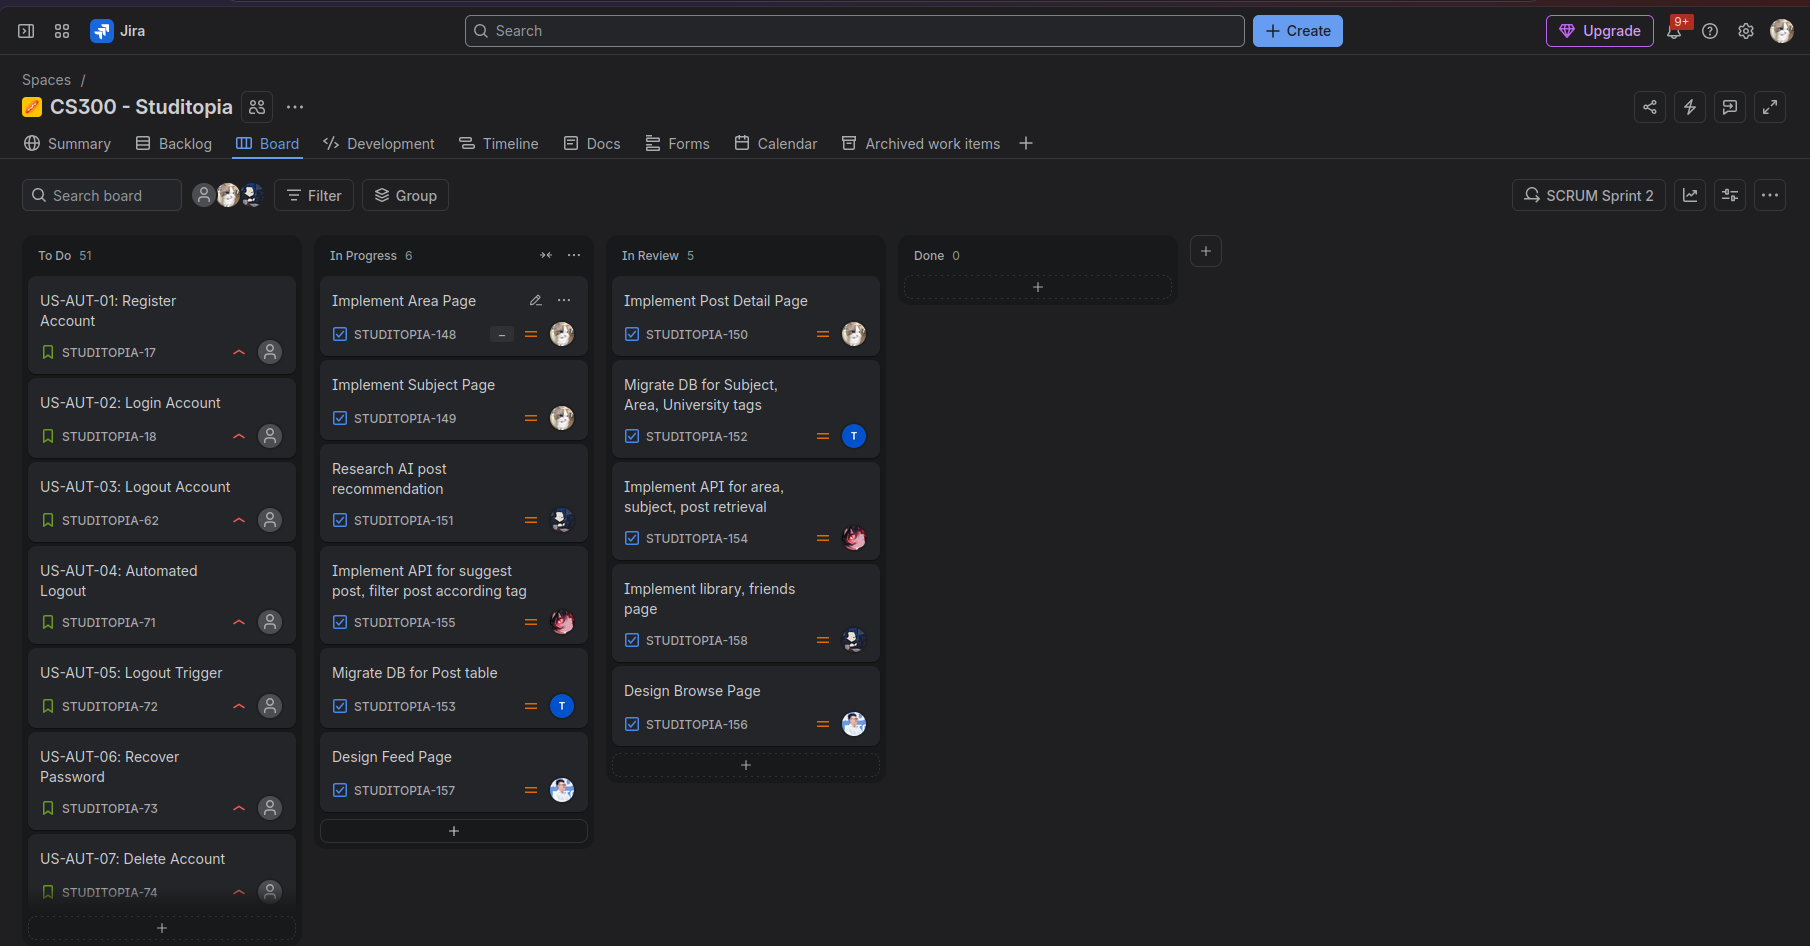
\includegraphics[width=0.8\linewidth]{images/jira_task_screen1.png}\caption{Jira task screenshot}\end{figure}

\end{document}
